\documentclass[11pt]{article}
\usepackage{graphicx}

\begin{document}
\title{Homework 16}
\author{Colt Bradley}
\date{}
\maketitle

\section{Exercise 1}

We compute the first derivative using the central difference method, which is represented by the following equation. 

\begin{equation}
f'(x) = \frac{f(x+h)-f(x-h)}{2h}
\end{equation}
Taking the ratio of $\frac{h_1^2}{h_2^2}$ values and error values $\frac{E_1}{E_2}$, we can see that these ratios match. We use $h_1 = .009$ and $h_2 = .01$. This implies that the error scales as $h^2$. 

\section{Exercise 2}
This time we use a five stencil, which takes the form of the following equation. 

\begin{equation}
f'(x) = af(x+2h)+bf(x+h)+cf(x)+df(x-h)+ef(x-2h)
\end{equation}

The coefficients $a, b, c, d,$ and $e$ can be determined through a system of equations. We do this inside of the defined function. Using the same ratio technique, we find that the error using this method goes as $h^4$. 
\section{Exercise 3}
For the final exercise, we calculate the second derivative of the function $\log(x)/\cosh(x)$ using the three point stencil that follows. 
\begin{equation}
f''(x) = \frac{f(x+h)-2f(x)+f(x-h)}{h^2}
\end{equation}

The error for this equation scales as $h^2$. A graph of the second derivative of the function in the interval $[2,5]$ is graphed, as well as the graph of the underlying function in the same interval. We can visually check this using what we know about calculus. 

\begin{figure}[ht]
\centering
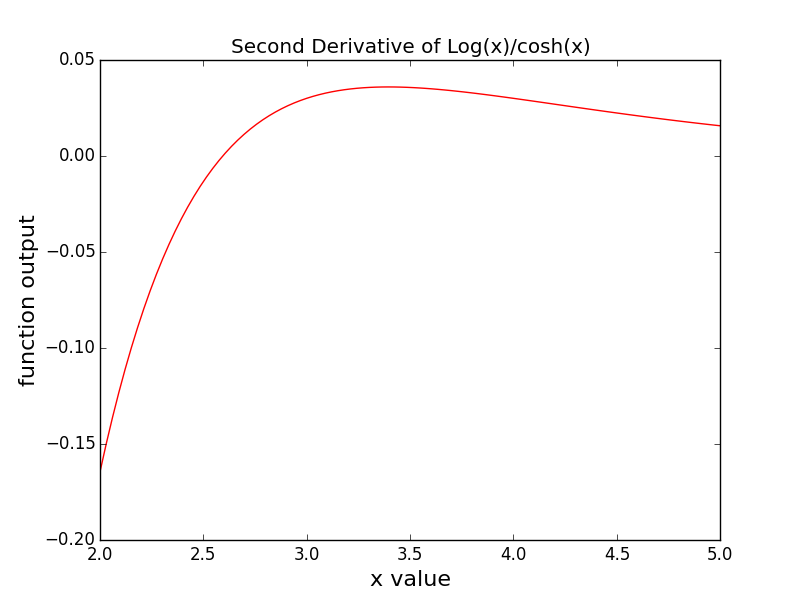
\includegraphics[scale=.4]{second_derivative.png}
\end{figure}

\begin{figure}[ht]
\centering
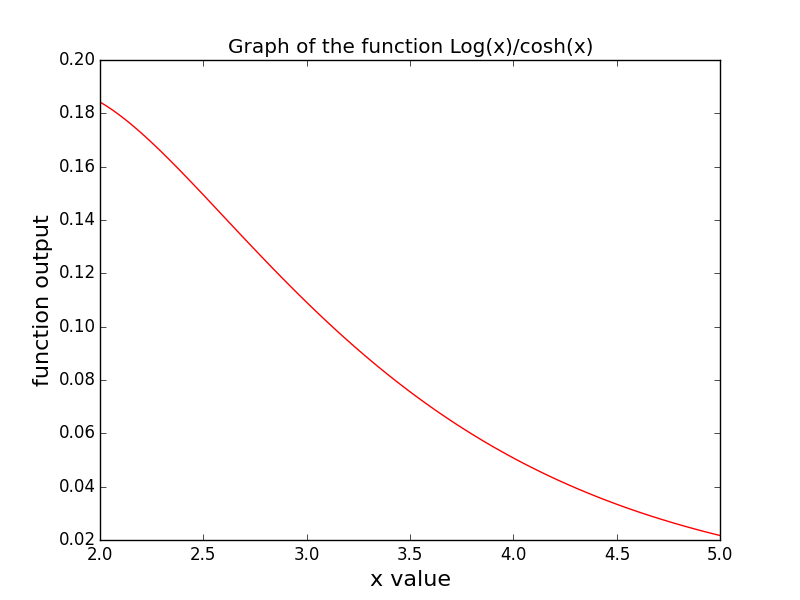
\includegraphics[scale=.4]{function.png}
\end{figure}

\section{Code}
\begin{verbatim}
#Colt Bradley
#3.17.16
#Lesson 16 Differentiation

#############################################################################
#functions and modules
#############################################################################
import numpy as n
import pylab as p

#function for exercise 1 and 2
def f(x):
    y = n.cos(x)*n.tanh(x)
    return y

#function for exercise 3
def g(x):
    y = n.log(x)/n.cosh(x)
    return y

#function to calculate central difference
def central_difference(f,x,h):
    deriv = (f(float(x+h))-f(float(x-h)))/(2.*h)
    return deriv

#This five stencil using linear algebra to solve for the coefficents
def five_stencil(f,x,h):
    x = float(x)
    h = float(h)
    big = n.matrix([[1,1,1,1,1],[-2,-1,0,1,2],\
[4,1,0,1,4],[-8,-1,0,1,8],[16,1,0,1,16]])
    col = n.matrix([[0],[1/h],[0],[0],[0]])
    ans = n.linalg.solve(big,col)
    deriv = ans.item(0)*f(x-2*h)+ans.item(1)*f(x-h)+ans.item(2)*f(x)+ \
    ans.item(3)*f(x+h)+ans.item(4)*f(x+2*h)
    return deriv
    
#absolute error calculating function
def error(val, expval):
    return (abs(val-expval)/expval)*100
    
#function to calculate central difference
def second_derivative(f,x,h):
    x = float(x)
    h = float(h)
    deriv = (f(float(x+h))+f(float(x-h))-2.*f(float(x)))/(h**2)
    return deriv

#############################################################################
#Exercise 1
#############################################################################
print "Exercise 1:"
#define initial values
h_1 = .009
h_2 = .01
x=2.

#calculate error using error function and compare
e_1 = error(central_difference(f,x,h_1),-0.905989)
e_2 = error(central_difference(f,x,h_2),-0.905989)
h_ratio = (h_1/h_2)**2
e_ratio = e_1/e_2
print "The ratio of h^2 values is {:.3f}. The ratio errors is {:.3f}. The ratio \
of the two is {:.3f} (closer to one means the error scales as h^2)\n" \
.format(h_ratio,e_ratio,h_ratio/e_ratio)

#############################################################################
#Exercise 2
#############################################################################
print "Exercise 2:"
#Define the matricies
h = .01
big = n.matrix([[1,1,1,1,1],[-2,-1,0,1,2],\
[4,1,0,1,4],[-8,-1,0,1,8],[16,1,0,1,16]])
col = n.matrix([[0],[1/h],[0],[0],[0]])

#use linear algebra package, print result
ans = n.linalg.solve(big,col)
#This is an example of what is encorperated into the function definition

print "The numerical aproximation to the derivative using a five-stencil is\
{:.3f}.\n".format(five_stencil(f,2,.01))
h_1 = .09
h_2 = .1
x=2. 

e_1 = error(five_stencil(f,x,h_1),-0.905989)
e_2 = error(five_stencil(f,x,h_2),-0.905989)
print "The ratio of h^4 values is {:.3f}. The ratio errors is {:.3f}. The\
ratio of the two is {:.3f} (closer to one means the error scales like h^4)\n" \
.format(h_ratio,e_ratio,h_ratio/e_ratio)

#############################################################################
#Exercise 3
#############################################################################
print "Exercise 3:"

#create a list to store the calculated values of the derivative and function
lst = n.linspace(2,5,100)
derivative = []
func = []

#list of derivative values
for i in lst:
    deriv = second_derivative(g,i,h)
    derivative.append(deriv)
    
#list of function values
for i in lst:
    k = g(i)
    func.append(k)

#plot of derivative
p.close()
p.plot(lst,derivative,"r")
p.title("Second Derivative of Log(x)/cosh(x)")
p.xlabel("x value",fontsize=16)
p.ylabel("function output",fontsize=16)
p.savefig("second_derivative.png")
p.show()

#plot of function
p.close()
p.plot(lst,func,"r")
p.title("Graph of the function Log(x)/cosh(x)")
p.xlabel("x value",fontsize=16)
p.ylabel("function output",fontsize=16)
p.savefig("function.png")
p.show()
\end{verbatim}


\end{document}